% diestel.tex

%%%%\definition{Ensembles séparables}
%%%%\label{separables}
%%%%	Etant donné un graphe $G = (V,E)$, deux sous-ensembles de sommets
%%%%	$Y,Z \subseteq V$ sont {\em séparables} si $|Y| = |Z|$ et
%%%%	$\exists S \subseteq V : |S| < |Y|$ tel que $G\setminus S$
%%%%	ne contient aucun chemin entre $Y \setminus S$ et $Z \setminus S$.

%%%%\definition{Ensemble k-lié}
%%%%\label{kconnected}
%%%%	Soit $G = (V,E)$ un graphe, un sous-ensemble de sommets
%%%%	$X \subseteq V$ est {\em k-lié} si $|X| \geq k$ et 
%%%%	$\forall Y,Z \subseteq V : |Y| = |Z| \leq k$, $Y$ et
%%%%	$Z$ sont non-séparables.

%%%%\theorem{Menger}
%%%%\label{thmenger}
%%%%	Soit $G = (V,E)$ un graphe.

\definition{Ensemble k-lié}
\label{kconnected}
	Etant donné un graphe $G = (V,E)$, un sous-ensemble de sommets $X \subseteq V$
	est {\em k-lié} si $|X| \geq k$ et $\forall Y,Z \subseteq V : |Y| = |Z| = n \leq k$,
	il existe $n$ chemins disjoints entre $Y$ et $Z$.

\definition{Ensemble k-lié externellement}
\label{kextconnected}
	Soit $G = (V,E)$ un graphe, un sous-ensemble de sommets $X \subseteq V$
	est {\em k-lié externellement} si $X$ est k-lié et de plus, les chemins n'utilisent
	aucune arête dans $E(X)$.

\proposition{(Diestel)}
\label{propdiestelh}
	Soient $G = (V,E)$ un graphe, $h \geq k \in \N^*$.\\
	Si $G$ ne contient aucun ensemble $k$-lié-externellement de taille $h$ alors,
	$tw(G) < h + k - 1$.

\preuve{propdiestelh}
	Soit $U \subseteq V$ maximal tel qu'il existe une décomposition
	arborescente ${\cal D} = (T,\{X_t : t \in T\})$ de largeur 
	$width({\cal D}) < h + k - 1$,
	telle que chaque composante $C$ connexe dans $G \setminus U$ a 
	au plus $h$ voisins, notés $\Gamma(C)$, dans $U$ et qu'il
	existe un n\oe ud $t \in T : \Gamma(C) \subseteq X_t$.
	\\
	{\em Hypothèse :} $U \neq V$.
	Soit $C$ une composante connexe de $G \setminus U$.
	On pose $X = \Gamma(C)$.
	\\
	On a $|X| \leq h$, on suppose $|X| < h$.
	Pour chaque sommet $v \in C$, on peut ajouter un n\oe ud $t$ dans
	$T$ tel que $X_t = X \cup \{v\}$, ainsi $U \cup \{x\}$ 
	contredit la maximalité de $U$.
	\\
	Donc $|X| = h$, et d'après l'hypothèse de la proposition
	$X$ n'est pas k-lié-externellement dans $G$.
	Soit $Y,Z \subseteq X$ les ensembles séparables de $X$ tels que
	$|Y| = |Z| = k$.
	% menger
	D'après le théorème de Menger \cite{thmenger}, il existe
	$S \subseteq C \cup Y \cup Z$ le séparateur de $Y,Z$ de taille $|S| < k$.
	On pose $X_Y = (X\setminus Z) \cup S$ et $X_Z = (X \setminus Y) \cup S$.
	On a $|X| = h \leq h + k -1$, et puisque $|S| < |Y|$, $|X_Y|,|X_Z| < |X| = h$.
	De plus, pour chaque composante $C' \subseteq C$ de $G \setminus (U\cup S)$,
	$\Gamma(C') \subseteq X \cup S$, et plus précisemment soit dans $X_Y$, soit dans
	$X_Z$ sinon il existe un chemin dans $X \setminus S$ reliant $Y$ et $Z$ à travers
	$C'$.
	Ainsi, $\Gamma(C') \subseteq X_Y$ ou bien $\Gamma(C') \subseteq X_Z$.
	\\
	Enfin, $S \cap C \neq \emptyset$ puisque $|S| < |Y|$.
	On peut donc étendre $U$ en ajoutant un n\oe ud $t$ tel que
	$X_t = X \cup S$ avec $|X_t| \leq h + k$ dans ${\cal D}$ contredisant l'hypothèse de maximalité
	de $U$.
	
\proposition{(Diestel)}
\label{propdiestel}
	Soient $G = (V,E)$ un graphe et $k \in \N^*$.
	\begin{itemize}
		\item[(i)] Si $tw(G) < k$ alors $G$ ne contient aucun ensemble
		$(k+1)$-lié de taille $n \geq 3k$.
		\item[(ii)] Si $G$ ne contient aucun ensemble $(k+1)$-lié externellement
		de taille $n \geq 3k$, alors $tw(G) < 4k$.
	\end{itemize}

\preuve{propdiestel}
	Soient $G = (V,E)$ un graphe et $k \in \N^*$.
	\begin{itemize}
		\item[(i)] 
		Soit $(T,\{X_t : t \in T\})$ une décomposition arborescente telle que $width(T) < k$.
		\\
		Soit $X \subseteq V$ un sous-ensemble des sommets de $G$ tel que $|X| \geq 3k$,
		et on suppose que $X$ est $(k+1)$-lié.
		Pour chaque arête $e = (t_1,t_2) \in E(T)$, soit $T'$ la composante de $T \setminus e$ telle que
		$|X \cap \bigcup\limits_{t\in T'}X_t|$ soit maximum, et $T''$ l'autre, on oriente $(t_1,t_2)$ de 
		de $T''$ vers $T'$.
		\\
		Soit un n\oe ud $t \in T$ tel que tous les arcs soient dirigés vers $t$.
		Pour chaque n\oe ud $t_1,...,t_\ell$ voisin de $t$, soit $(A_i,B_i)$ une
		séparation correspondante de $t_i$ telle que $X_t \subseteq B_i$.\\
		{\em Hypothèse :} $|A_i \cap X| \geq k$.\\
		On a alors par construction $|B_i \cap X| \geq k$, ainsi on peut trouver
		$Y \subseteq A_i \cap X$ et $Z \subseteq B_i \cap X$ tels que $|Y| = |Z| = k$.
		Or, $S = A_i \cap B_i$ sépare $A_i$ et $B_i$, donc également $Y$ et $Z$, de
		plus $|S| < k$, contredisant le fait que $X$ soit $(k+1)$-lié (figure \ref{fig_aicapx}).
		\\
		% aicapx.tex

\begin{figure}[!ht]
\begin{center}
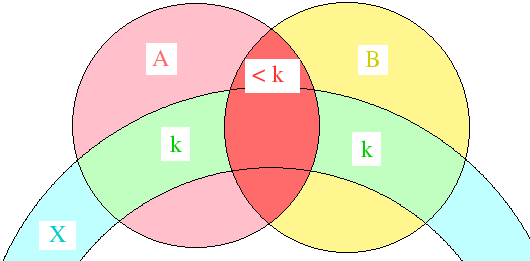
\includegraphics[scale=0.5]{res/aicapx}
\end{center}
\caption{illustration preuve \ref{propdiestel} : hypothèse $A_i \cap X \geq k$}
\label{fig_aicapx}
\end{figure}


		Ainsi, $|A_i \cap X| < k$.
		\\
		Soit $i \in [\ell]$ minimal tel que $|(A_1 \cup ... \cup A_i) \cap X| > k$.
		On pose $A = \bigcup\limits_{j \in [i]} A_j$ et 
		$B = \bigcup\limits_{j\in [i]} B_j$.
		Puisque $i$ est minimal et $|A_i \cap X| < k$ on a $|A \cap X| < 2k$.
		Et donc $|B\cap X| > |X| - 2k \geq k$.
		Soient $Y \subseteq A \cap X, Z \subseteq B\cap X$ tels que
		$|Y| = |Z| = k$.
		Or par la proposition \ref{xsep} $X_t$ est un séparateur de $Y$ et $Z$
		de taille $ < k$.
		Ce qui est en contradiction avec l'hypothèse que $X$ est un ensemble
		$(k+1)$-lié (figure \ref{fig_aicapx2}).
		\\
		% aicapx2.tex

\begin{figure}[H]
\begin{center}

\begin{tikzpicture}[]
	\node [vertex,fill=green!50] (v0) {};
	\node [vertex] (v1) [below of=v0] {};
	\node [vertex,fill=green!50] (v2) [right of=v0] {};
	\node [vertex,fill=green!50] (v3) [right of=v1] {};
	\node [vertex,fill=green!50] (v4) [right of=v3] {};
	\node [vertex,fill=green!50] (v5) [below of=v3] {};
	\node [vertex] (v6) [below of=v4] {};
	\node [vertex] (v7) [below right of=v5] {};
	\node [vertex,fill=green!50] (v8) [right of=v4] {};
	\node [vertex] (v9) [above right of=v4] {};
	\node [vertex] (v10) [above left of=v9] {};
	\node [label] (lv0) at (1,0.5) {{\Large \color{green!66!black} $X$}};

	\draw [edge] (v0) -- (v1);
	\draw [edge] (v0) -- (v2);
	\draw [edge] (v1) -- (v3);
	\draw [edge] (v2) -- (v3);
	\draw [edge] (v2) -- (v4);
	\draw [edge] (v2) -- (v9);
	\draw [edge] (v2) -- (v10);
	\draw [edge] (v3) -- (v4);
	\draw [edge] (v3) -- (v5);
	\draw [edge] (v4) -- (v6);
	\draw [edge] (v4) -- (v8);
	\draw [edge] (v4) -- (v9);
	\draw [edge] (v5) -- (v6);
	\draw [edge] (v5) -- (v7);
	\draw [edge] (v6) -- (v7);
	\draw [edge] (v8) -- (v9);
	\draw [edge] (v9) -- (v10);

	\node [treedec] (t0) at (1,-1) {};
	\node [treedec,fill=green!50] (t1) at (2.7,-1.3) {};
	\node [treedec] (t2) at (3,-3) {};
	\node [treedec] (t3) at (3.2,-4.5) {};
	\node [treedec] (t4) at (4,-1) {};
	\node [treedec] (t5) at (5.25,-1.5) {};
	\node [treedec] (t6) at (4,0.25) {};
	\node [label] (lt0) at (0.5,-0.5) {{\Large \color{red} $T$}};

	\draw [treeedge,->,ultra thick] (t0) -- (t1);
	\draw [treeedge,<-,ultra thick] (t1) -- (t2);
	\draw [treeedge,<-,ultra thick] (t1) -- (t4);
	\draw [treeedge,<-,ultra thick] (t2) -- (t3);
	\draw [treeedge,<-,ultra thick] (t4) -- (t5);
	\draw [treeedge,<-,ultra thick] (t4) -- (t6);
% TODO séparations Ai, Bi, A, B
	\draw [separator] (2.1,1) -- (2.1,-2) -- (0.3,-3.7);
	\node [label] (ls1a) at (0.7,-2.7) {{\Large \color{blue} $A_1$}};
	\node [label] (ls1b) at (1.3,-3.3) {{\Large \color{blue} $B_1$}};
	\draw [separator] (1.7,0.4) -- (5.4,-3.3);
	\node [label] (ls2a) at (5,-2.4) {{\Large \color{blue} $A_2$}};
	\node [label] (ls2b) at (4.5,-3) {{\Large \color{blue} $B_2$}};
	\draw [separator] (-0.5,-1.9) -- (6.8,-1.9);
	\node [label] (ls3a) at (6.5,-2.2) {{\Large \color{blue} $A_3$}};
	\node [label] (ls3b) at (6.5,-1.6) {{\Large \color{blue} $B_3$}};

\end{tikzpicture}

\begin{tikzpicture}[]
	\node [vertex,fill=blue!50] (v0) {};
	\node [vertex] (v1) [below of=v0] {};
	\node [vertex,fill=blue!50,draw=green] (v2) [right of=v0] {};
	\node [vertex,fill=blue!50,draw=green] (v3) [right of=v1] {};
	\node [vertex,fill=blue!50,draw=green] (v4) [right of=v3] {};
	\node [vertex,fill=yellow!50] (v5) [below of=v3] {};
	\node [vertex] (v6) [below of=v4] {};
	\node [vertex] (v7) [below right of=v5] {};
	\node [vertex,fill=blue!50] (v8) [right of=v4] {};
	\node [vertex] (v9) [above right of=v4] {};
	\node [vertex] (v10) [above left of=v9] {};
	\node [label] (lv0) at (1,0.5) {{\Large \color{green!66!black} $X$}};

	\draw [edge] (v0) -- (v1);
	\draw [edge] (v0) -- (v2);
	\draw [edge] (v1) -- (v3);
	\draw [edge,draw=green] (v2) -- (v3);
	\draw [edge,draw=green] (v2) -- (v4);
	\draw [edge] (v2) -- (v9);
	\draw [edge] (v2) -- (v10);
	\draw [edge,draw=green] (v3) -- (v4);
	\draw [edge] (v3) -- (v5);
	\draw [edge] (v4) -- (v6);
	\draw [edge] (v4) -- (v8);
	\draw [edge] (v4) -- (v9);
	\draw [edge] (v5) -- (v6);
	\draw [edge] (v5) -- (v7);
	\draw [edge] (v6) -- (v7);
	\draw [edge] (v8) -- (v9);
	\draw [edge] (v9) -- (v10);

	\node [treedec] (t0) at (1,-1) {};
	\node [treedec,fill=green!50] (t1) at (2.7,-1.3) {};
	\node [treedec] (t2) at (3,-3) {};
	\node [treedec] (t3) at (3.2,-4.5) {};
	\node [treedec] (t4) at (4,-1) {};
	\node [treedec] (t5) at (5.25,-1.5) {};
	\node [treedec] (t6) at (4,0.25) {};
	\node [label] (lt0) at (0.5,-0.5) {{\Large \color{red} $T$}};

	\draw [treeedge,->,ultra thick] (t0) -- (t1);
	\draw [treeedge,<-,ultra thick] (t1) -- (t2);
	\draw [treeedge,<-,ultra thick] (t1) -- (t4);
	\draw [treeedge,<-,ultra thick] (t2) -- (t3);
	\draw [treeedge,<-,ultra thick] (t4) -- (t5);
	\draw [treeedge,<-,ultra thick] (t4) -- (t6);
% TODO séparations Ai, Bi, A, B
	\draw [separator] (2.1,1) -- (2.1,-2) -- (0.3,-3.7);
	\node [label] (ls1a) at (0.7,-2.7) {{\Large \color{blue} $A_1$}};
	\node [label] (ls1b) at (1.3,-3.3) {{\Large \color{blue} $B_1$}};
	\draw [separator] (1.7,0.4) -- (5.4,-3.3);
	\node [label] (ls2a) at (5,-2.4) {{\Large \color{blue} $A_2$}};
	\node [label] (ls2b) at (4.5,-3) {{\Large \color{blue} $B_2$}};
	\draw [separator] (-0.5,-1.9) -- (6.8,-1.9);
	\node [label] (ls3a) at (6.5,-2.2) {{\Large \color{blue} $A_3$}};
	\node [label] (ls3b) at (6.5,-1.6) {{\Large \color{blue} $B_3$}};

	\node [label] (ltA) at (0,0.5) {{\Large \color{blue!66!black} $A$}};
	\node [label] (ltB) at (1.5,-4.5) {{\Large \color{yellow!50!black} $B$}};


\end{tikzpicture}

\end{center}
\caption{illustration preuve \ref{propdiestel} : hypothèse $A_i \cap X < k$
chaque sommet représente un sous-graphe connexe de taille $\frac{k}{4}$}
\label{fig_aicapx2}
\end{figure}


		
		\item[(ii)]
		En appliquant la proposition \ref{propdiestelh} pour $h = 3k$, le résultat est immédiat.


	\end{itemize}

